\section{Positivity Constraint} \label{sec:posconst}
\subsection{Matrix Quantity}
This section particularly explains the reconstruction of the 3D electron density from the \Blq. The essential treatmeant of this methos is to convert all quantities into a matrix or vector. 

The first step is to find the estimate of $I_{lm}(q)$. The singular values decomposition (SVD) of the \Blq can be used to get an estimate of \Ilm. From equation \ref{eq:svdilm}, SVD on the \Blq for particular $l$ is performed and the nonuniqueness of \Ilm originate from unitary matrix $O^{\dagger}$. The derivation is  

\begin{align}
B_{l}(q,q') &= UDU^{t} \\
B_{l}(q,q') &= U\sqrt{D} O^{\dagger} O \sqrt{D} U^{t}  \\
I_{lm}(q)  &= (U \sqrt{D}) O^{\dagger}. 
\label{eq:svdilm}
\end{align}

One can shows that the \Ilm on equation \ref{eq:svdilm} is already in matrix form. For the reason of clarity in the indices, a new matrix $G$ are defined in equation \ref{eq:gmatrix}. The matrix $G$ is the first estimate of \Ilm and the actual solution of \Ilm has dependence on $O^{\dagger}$.  The rows correspond to $q$ coordinate and the columns correspond $m$ value, or the singular values in the symmetric case. For the asymmetric case, there will be $2l+1$ columns in matrix $G$ whereas for 4-fold symmetry the number of column for each $l$ is shown in figure \ref{fig:4foldsvd}. Additionally, the matrix $G$ is in a form of multiplication between $U$, which is eigenvector of the \Blq, and $\sqrt{D}$, which is diagonal matrix consist of the singular values of the \Blq. In general:

\begin{eqnarray}
G=U \sqrt{D}
\label{eq:gmatrix}
\end{eqnarray}
\begin{eqnarray*}
  \begin{pmatrix}
    I_{l(-l)}(q_{1})&\dots&I_{l(l)}(q_{1})\\
    I_{l(-l)}(q_{2})&\dots&I_{l(l)}(q_{2})\\
    I_{l(-l)}(q_{3})&\dots&I_{l(l)}(q_{3})\\
    \vdots&\vdots&\vdots& \\
    I_{l(-l)}(q_{N})&\dots&I_{l(l)}(q_{N})\\
  \end{pmatrix}
    =
\label{eq:ilmmatrix}
\end{eqnarray*}
\begin{eqnarray}
  \begin{pmatrix}
    G^{l}_{1(-l)}&G^{l}_{1(-l+1)}&\dots&G^{l}_{1(l)}
\\
    G^{l}_{2(-l)}&G^{l}_{2(-l+1)}&\ldots&G^{l}_{2(l)}
\\
    \vdots&\vdots&\vdots&\vdots \\
    G^{l}_{N(-l)}&G^{l}_{N(-l+1)}&\ldots&G^{l}_{N(l)}
  \end{pmatrix}
  \begin{pmatrix}
    O^{l}_{1(-l)}&O^{l}_{1(-l+1)}&\ldots&O^{l}_{1(l)}\\
    O^{l}_{2(-l)}&O^{l}_{2(-l+1)}&\ldots&O^{l}_{2(l)} \\
    \vdots&\vdots&\vdots&\ldots \\
    O^{l}_{(l)(-l)}&O^{l}_{(l)(-l+1)}&\ldots&O^{l}_{(l)(l)} \\
  \end{pmatrix}
\label{eq:gmatrixO}
\end{eqnarray}

The Full \Ilm matrix is shown in equation \ref{eq:ilmmatrix}. The rows correspond to $q$ coordinate and columns correspond to $m$ values. The matrix in equation \ref{eq:gmatrixO} is an example of how multiplication occur on the matrix $G$ and $O^{l}_{mm'}$. Depending on the symmetry, in general the matrix $O^{l}_{mm}$ have the dimension $2l+1$ by $2l+1$. The goal of this method is to find the matrix $O^{l}_{mm'}$ by any constraint other than \Blq    

In order to use positivity constraint, the relation between $I(\vec{q})$, \Blq, and $O^{l}_{mm'}$ is needed. $I(\vec{q})$ can be found by substituting \Ilm to its spherical harmonics expansion. Shown in equation \ref{eq:Iqilm}, $I(\vec{q})$ can be related to the matrix $G$, $O^{l}_{mm'}$, and $Y_{lm}(\Omega)$. 

\begin{eqnarray}
I_{lm}(q_{1})&=&\sum_{m'} G^{l}_{1(m')} O^{l}_{i(m)} \\
I(q_{1},\Omega_{1})&=&\sum_{lm} I_{lm}(q_{1}) Y_{lm}(\Omega_{1}) \\
I(q_{1},\Omega_{1})&=&\sum_{lmm'} G^{l}_{1(m')} O^{l}_{m'(m)} Y_{lm}(\Omega_{1})  
\label{eq:Iqilm}
\end{eqnarray}

It is important to note that equation \ref{eq:Iqilm} is a form of a linear equation. The property of many linear equations is it can be separated between known and unknown quantity. In this case the matrix $G$ and $Y_{lm}(\Omega)$ are known quantity where as matrix $O^{l}_{mm'}$ is unknown quantity. The separation is constructed by creating matrix consist of several linear equations. Equation \ref{eq:Iqgomatrix} is the matrix constructed from linear equation of $I(\vec{q})$ at different $q$ point.  
\begin{eqnarray}
\begin{pmatrix}
I(q_{1}) \\
I(q_{2}) \\
\ldots \\
I(q_{n}) 
\end{pmatrix}
\label{eq:Iqgomatrix}
= 
\end{eqnarray}
\begin{eqnarray*}
\begin{pmatrix}
G^{0}_{1(0)} Y_{00} & G^{2}_{1(-2)} Y_{2(-2)} & \ldots & G^{2}_{1(2)} Y_{2(2)} & G^{4}_{1(-4)} Y_{4(-4)} & \dots  & G^{4}_{1(4)}Y_{(4)(-4)} \\
G^{0}_{1(0)} Y_{00} & G^{2}_{1(-2)} Y_{2(-2)} & \ldots & G^{2}_{1(2)} Y_{2(2)} & G^{4}_{1(-4)} Y_{4(-4)} & \dots  & G^{4}_{1(4)}Y_{(4)(-4)} \\
\ldots & \ldots & \ldots & \ldots & \\
G^{0}_{N(0)} Y_{00} & G^{2}_{N(-2)} Y_{2(-2)} & \ldots & G^{2}_{N(2)} Y_{2(2)} & G^{4}_{N(-4)} Y_{4(-4)} & \dots  & G^{4}_{1(4)}Y_{(4)(-4)} \\
\end{pmatrix}
\begin{pmatrix}
O^{0}_{1(0)} \\
O^{2}_{(-2)(-2)} \\
\vdots \\
O^{2}_{(2)(2)} \\
O^{4}_{(4)(-4)} \\
\vdots \\
O^{4}_{(4)(4)} \\
\vdots \\
\end{pmatrix}
\end{eqnarray*}

To be more concise, a new definition of the matrix $C$ and the vector $V$ is made. The matrix $C$ is multiplication between $G$ and $Y_{lm}$. The vector $V$ is one dimensional vector which consist of element or unitary matrix $O^{l}_{mm'}$. 
\begin{equation}
\label{eq:Cmatrix}
C=
\begin{pmatrix}
G^{0}_{1(0)} Y_{00} & G^{2}_{1(-2)} Y_{2(-2)} & \ldots & G^{2}_{1(2)} Y_{2(2)} & G^{4}_{1(-4)} Y_{4(-4)} & \dots  & G^{4}_{1(4)}Y_{(4)(-4)} \\
G^{0}_{1(0)} Y_{00} & G^{2}_{1(-2)} Y_{2(-2)} & \ldots & G^{2}_{1(2)} Y_{2(2)} & G^{4}_{1(-4)} Y_{4(-4)} & \dots  & G^{4}_{1(4)}Y_{(4)(-4)} \\
\ldots & \ldots & \ldots & \ldots & \\
G^{0}_{N(0)} Y_{00} & G^{2}_{N(-2)} Y_{2(-2)} & \ldots & G^{2}_{N(2)} Y_{2(2)} & G^{4}_{N(-4)} Y_{4(-4)} & \dots  & G^{4}_{1(4)}Y_{(4)(-4)} \\
\end{pmatrix} \\
\end{equation}
\begin{equation}
\label{eq:Vvector}
\vec{V}=
\begin{pmatrix}
O^{0}_{1(0)} \\
O^{2}_{(-2)(-2)} \\
\vdots \\
O^{2}_{(2)(2)} \\
O^{4}_{(4)(-4)} \\
\vdots \\
O^{4}_{(4)(4)} \\
\vdots \\
\end{pmatrix}
\end{equation}
Equation \ref{eq:IqtoOrtho} is a matrix relation which relate between the intensity and \Blq. The information about \Blq is retained inside matrix $C$ that comes from SVD of \Blq. The vector $V$ is giving the nonuniqueness of intensity from \Blq data since its elements consist of element of unitary matrix $O^{l}_{mm'}$. 

Important to note that the relation, which is based on equation \ref{eq:IqtoOrtho}, can be used to check whether the intensity satisfy \Blq constraint or not. If the data of intensity is available, then by taking the inverse matrix $C$, which is multiplied by the intensity, a new vector $V$ can be calculated. If the new vector $V$ consist of element of unitary matrix then that intensity satisfy \Blq constraint. However if elements of the new vector $V$ doesn't have the property of unitary matrix then that intensity doesn't satisfy \Blq constraint. 
\begin{eqnarray}
\label{eq:IqtoOrtho}
I(\vec{q},\Omega) = C V 
\end{eqnarray}

\subsection{Optimization}
As mentioned in previous section, the intensity is always positive because it is square absolute value of the amplitude. This fact can be used to limit the possibility o the solution and resolve the nonuniqueness of unitary matrix $O^{l}_{mm'}$. The optimization can be used to constraint the intensity to be positive and at the same time satisfy requirement \Blq. 

There is optimization algorithm that is suitable for constraining positive solution and satisfy the objective function at the same time, which is called active set, its definition is
\begin{eqnarray}
\mbox{minimize}\quad f(x) \\ \nonumber
\quad \mbox{subject to} \quad Ax\geq b
\label{eq:activealgo}
\end{eqnarray}
According to equation \ref{eq:IqtoOrtho}, variables in equation \ref{eq:activealgo} need to be adjusted. In this case, $b=0$, $x=V$, and $A=C$ to satisfy the positivity constraint. 

From equation \ref{eq:svdilm}, as long as $O^{l}_{mm'}$ is unitary matrix then \Blq constraint is satisfied. Based on that requirement, the objective function $f(x)$ in equation \ref{eq:activealgo} is such that the matrix $O^{l}_{mm'}$ is unitary.  

Mathematically, unitary matrix is
\begin{eqnarray}
O^{l}_{mm'} (O^{l}_{mm'})^{\dagger} = 1. 
\end{eqnarray}
By defining new quantity,
\begin{eqnarray}
N^{l}_{nn'}=\sum_{m} O^{l}_{nm} (O^{l}_{n'm})^{\dagger} \\ \nonumber
\label{eq:NOmatrix}
\begin{pmatrix}
N^{l}_{(-l)(-l)}&N^{l}_{(-l)(-l+1)}&\dots&N^{l}_{(-l)(l)} \\
N^{l}_{(-l+1)(-l)}&N^{l}_{(-l+1)(-l+1)}&\dots&N^{l}_{(-l+1)(l)} \\
\vdots&\vdots&\vdots&  \\
N^{l}_{(l)(-l)}&N^{l}_{(l)(-l+1)}&\dots&N^{l}_{(l)(l)}
\end{pmatrix}
=
\begin{pmatrix}
1&0&\dots&0 \\
0&1&\dots&0 \\
\vdots&\vdots&\vdots&  \\
0&0&\dots&1 \\
\end{pmatrix}
\end{eqnarray}
If matrix $N^{l}_{nn'}$ is identity matrix then following is satisfied
\begin{eqnarray}
\sum_{n,n',l}(N^{l}_{nn'}-\delta_{n,n'})^2=0 \\
\mbox{where} \quad \delta_{n,n'} \quad \mbox{is Kronecker delta } \nonumber
\label{eq:objfunN}
\end{eqnarray}

Equation \ref{eq:objfunN} can be used as objective function. The objective function here is to ensure \Blq is satisfied or in other words matrix $O^{l}_{mm'}$ is unitary. The matrix $O^{l}_{mm'}$ is unitary if $N^{l}_{nn'}$ is identity matrix based on equation \ref{eq:NOmatrix}. As a consequence of that, if equation \ref{eq:objfunN} is satisfied then \Blq constraint is satisfied as well. 
The definition of objective function is written in full way that is
\begin{eqnarray}
\mbox{minimize}\quad \sum_{n,n',l}(N^{l}_{nn'}-\delta_{n,n'})^2 \\
\mbox{where} \quad N^{l}_{nn'}=\sum_{m} O^{l}_{nm}(O^{l}_{n'm})^{\dagger} \\
\quad \mbox{subject to} \quad  I(\vec{q})=C V \geq 0
\label{eq:optiOlm}
\end{eqnarray}
Built in function in matlab is used to perform optimization with active set algorithm. In matlab command, active set is in under command \textit{fmincon}.  
\begin{figure}[h!]
  \centering
  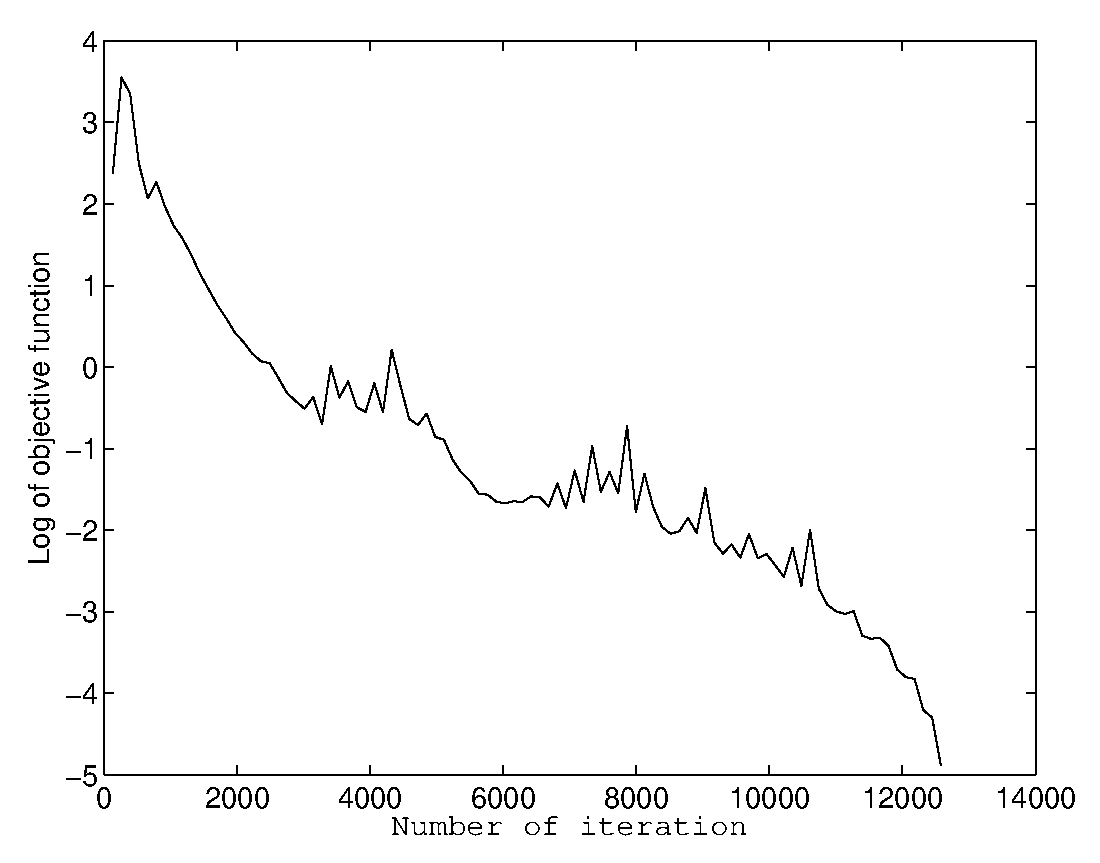
\includegraphics[width=.7\textwidth]{logobj}
\caption{Log of objective function vs number of iteration}
\label{fig:objfun}
\end{figure}
\begin{figure}[h!]
  \centering
  \includegraphics[width=.4\textwidth]{kccorner}
\caption{reconstruction of electron density}
\label{fig:receden}
\end{figure}

The simulation was done by calculating \Blq of K channel protein. After \Blq of K channel protein was calculated then optimization based on equation \ref{eq:optiOlm} was used.  Graph on figure \ref{fig:objfun} is the plot of $log$ of the objective function vs number of iteration. It is obvious from graph that by the end of iteration the objective function is reaching $10^{-6}$, which is small enough or approaching zero. In other words, by objective function is zero then requirement matrix $O^{l}_{mm'}$ is unitary is satisfied.  
\begin{figure}[h!]
  \centering
  \includegraphics[width=.5\textwidth]{BlcompL2}
\caption{Validation model and its reconstruction}
\label{fig:valmodrec2}
\end{figure}
\begin{figure}[h!]
\begin{subfigure}{.5\textwidth}
  \centering
  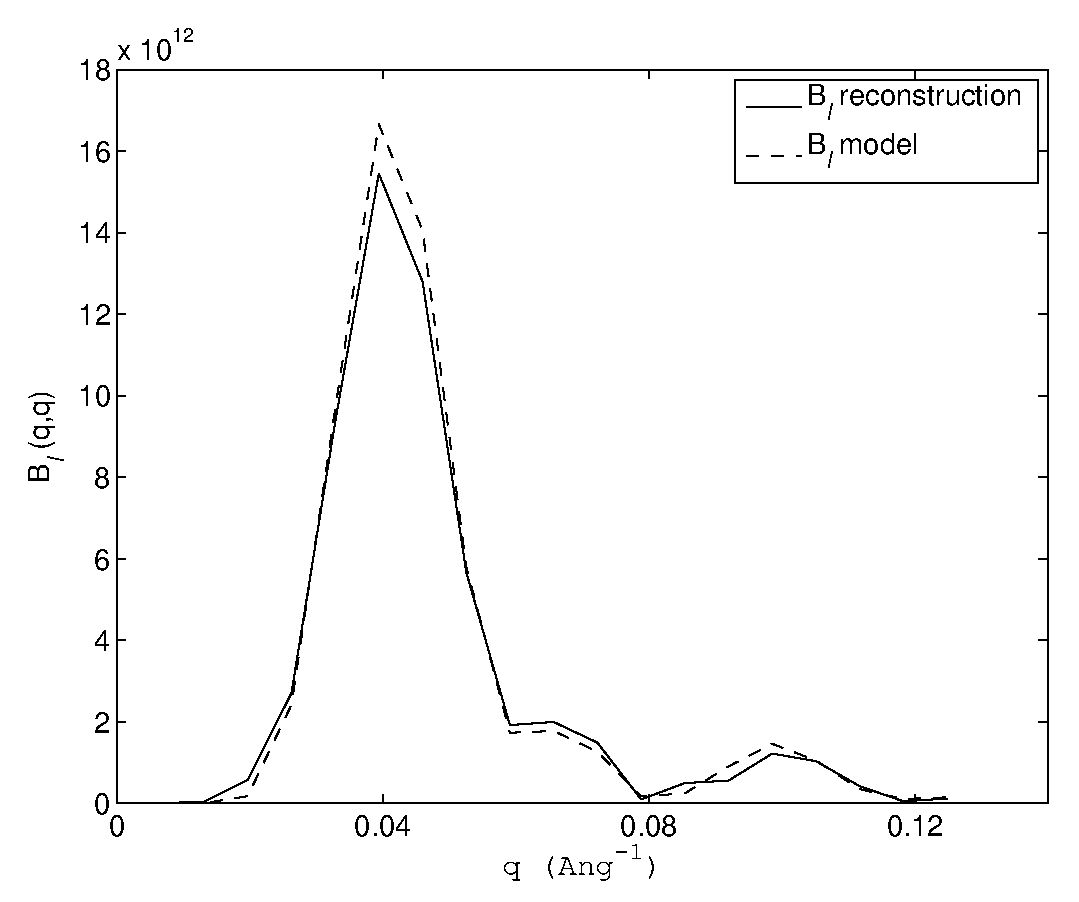
\includegraphics[width=1.0\textwidth]{BlcompL10}
  \caption{$l=10$}
\end{subfigure}
\begin{subfigure}{.5\textwidth}
  \centering
  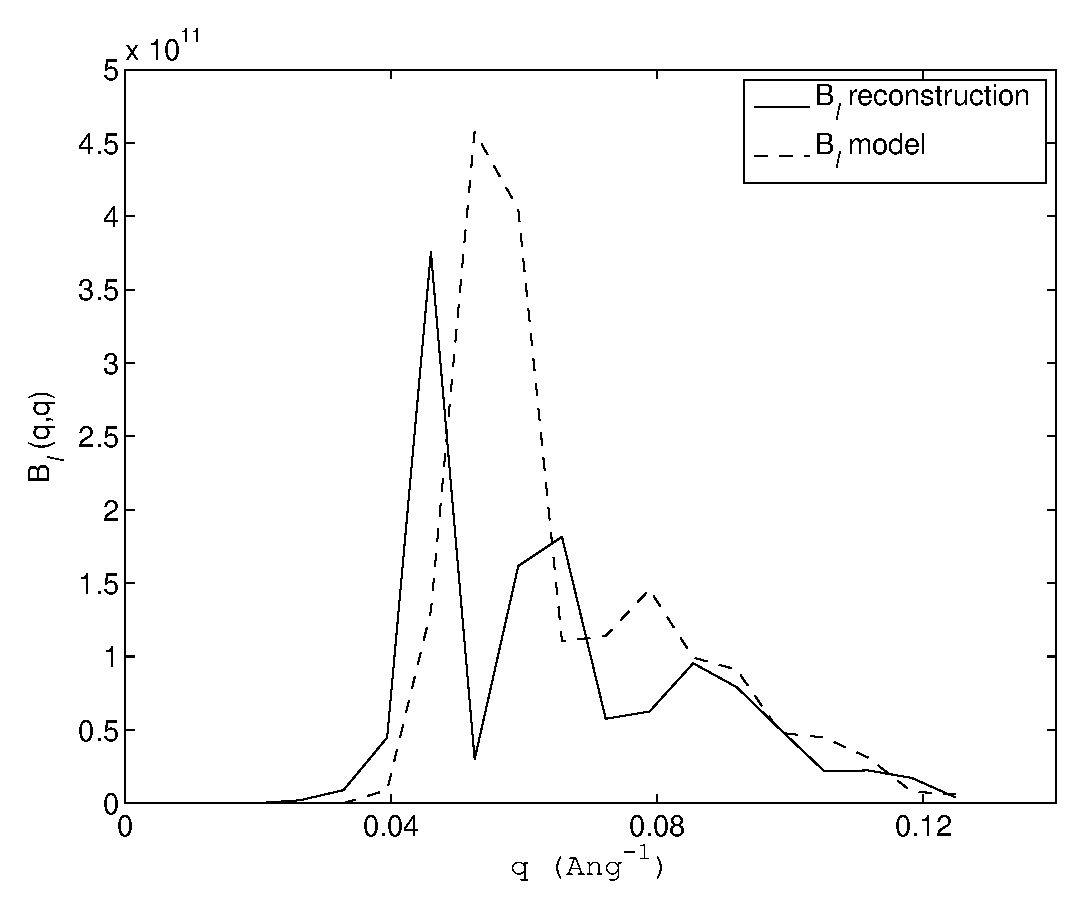
\includegraphics[width=1.0\textwidth]{BlcompL16}
  \caption{$l=16$}
\end{subfigure}
\caption{Validation model and its reconstruction}
\label{fig:valrec1016}
\end{figure}

After the intensity was reconstructed, the electron density was obtained by using charge flipping algorithm. Figure \ref{fig:receden} are electron density  after phasing algorithm. It has 4-fold symmetry and it enclose the original model. To test how valid the reconstruction is, \Blq is compared between model and reconstruction. It is shown in graph on figure \ref{fig:valmodrec2} and \ref{fig:valrec1016}, that reconstruction can recover \Blq for $l=2$ and $l=10$. However from $l=16$, \Blq begin to deviate from original model. Currently that is the limit of this method since the method only considers positivity constraint. There is other constraint that is not considered namely real space constraint on electron density. The explanation of real space constraint is given in chapter \ref{ch:futureimp}  


